% Options for packages loaded elsewhere
\PassOptionsToPackage{unicode}{hyperref}
\PassOptionsToPackage{hyphens}{url}
\PassOptionsToPackage{dvipsnames,svgnames,x11names}{xcolor}
%
\documentclass[
]{article}
\usepackage{amsmath,amssymb}
\usepackage{iftex}
\ifPDFTeX
  \usepackage[T1]{fontenc}
  \usepackage[utf8]{inputenc}
  \usepackage{textcomp} % provide euro and other symbols
\else % if luatex or xetex
  \usepackage{unicode-math} % this also loads fontspec
  \defaultfontfeatures{Scale=MatchLowercase}
  \defaultfontfeatures[\rmfamily]{Ligatures=TeX,Scale=1}
\fi
\usepackage{lmodern}
\ifPDFTeX\else
  % xetex/luatex font selection
\fi
% Use upquote if available, for straight quotes in verbatim environments
\IfFileExists{upquote.sty}{\usepackage{upquote}}{}
\IfFileExists{microtype.sty}{% use microtype if available
  \usepackage[]{microtype}
  \UseMicrotypeSet[protrusion]{basicmath} % disable protrusion for tt fonts
}{}
\makeatletter
\@ifundefined{KOMAClassName}{% if non-KOMA class
  \IfFileExists{parskip.sty}{%
    \usepackage{parskip}
  }{% else
    \setlength{\parindent}{0pt}
    \setlength{\parskip}{6pt plus 2pt minus 1pt}}
}{% if KOMA class
  \KOMAoptions{parskip=half}}
\makeatother
\usepackage{xcolor}
\usepackage[margin=1in]{geometry}
\usepackage{graphicx}
\makeatletter
\def\maxwidth{\ifdim\Gin@nat@width>\linewidth\linewidth\else\Gin@nat@width\fi}
\def\maxheight{\ifdim\Gin@nat@height>\textheight\textheight\else\Gin@nat@height\fi}
\makeatother
% Scale images if necessary, so that they will not overflow the page
% margins by default, and it is still possible to overwrite the defaults
% using explicit options in \includegraphics[width, height, ...]{}
\setkeys{Gin}{width=\maxwidth,height=\maxheight,keepaspectratio}
% Set default figure placement to htbp
\makeatletter
\def\fps@figure{htbp}
\makeatother
\setlength{\emergencystretch}{3em} % prevent overfull lines
\providecommand{\tightlist}{%
  \setlength{\itemsep}{0pt}\setlength{\parskip}{0pt}}
\setcounter{secnumdepth}{-\maxdimen} % remove section numbering
\ifLuaTeX
  \usepackage{selnolig}  % disable illegal ligatures
\fi
\IfFileExists{bookmark.sty}{\usepackage{bookmark}}{\usepackage{hyperref}}
\IfFileExists{xurl.sty}{\usepackage{xurl}}{} % add URL line breaks if available
\urlstyle{same}
\hypersetup{
  colorlinks=true,
  linkcolor={Maroon},
  filecolor={Maroon},
  citecolor={Blue},
  urlcolor={blue},
  pdfcreator={LaTeX via pandoc}}

\author{}
\date{\vspace{-2.5em}}

\begin{document}

\hypertarget{scratch-countdown-spirals}{%
\section{Scratch: Countdown Spirals}\label{scratch-countdown-spirals}}

\includegraphics{scratch_files/figure-latex/unnamed-chunk-1-1.pdf}

Remember the countdown spirals? In the example below, the pen moves 16
units, then 15 units, then 14 units, and the segments get smaller and
smaller down to 1 unit, after which the next segment is 16 units, then
15 units, etc\ldots{} and after each segment the direction is changed by
72°.


\includegraphics{scratch_files/figure-latex/unnamed-chunk-2-1.pdf}

Our goal is to produce these patterns in Scratch. You will
\textbf{submit a slideshow} with a variety of your best results. You
need to have at least 6 high-quality images of distinct spiral patterns
for full credit. Each image should also show the parameter settings used
to generate the image.

\begin{enumerate}
\def\labelenumi{\arabic{enumi}.}
\tightlist
\item
  Go to \href{https://scratch.mit.edu}{scratch.mit.edu}

  \begin{itemize}
  \tightlist
  \item
    Login (to save your work)
  \item
    \textbf{Create a new project} (click ``Create'' near top of page.)
  \end{itemize}
\item
  Click ``Add Extension'' button (bottom left of screen).
  
\includegraphics[width=0.05\textwidth,height=\textheight]{add_extension.png}

  \begin{itemize}
  \tightlist
  \item
    Choose the \textbf{Pen extension}.
  \end{itemize}
\item
  Make some variables.

  \begin{itemize}
  \tightlist
  \item
    On left side, click the ``Variables'' section of code. (The orange
    dot.)
  \item
    For each variable we need, click ``Make a Variable'', and then type
    the variable name.
  \item
    \textbf{Make 7 variables}:

    \begin{itemize}
    \tightlist
    \item
      \color{red}\texttt{x\_initial}\color{black}: the \(x\) coordinate
      to start the drawing.
    \item
      \color{red}\texttt{y\_initial}\color{black}: the \(y\) coordinate
      to start the drawing.
    \item
      \color{red}\texttt{direction\_initial}\color{black}: the direction
      to move at start of drawing.
    \item
      \color{red}\texttt{scale}\color{black}: a multiplier to make
      drawing bigger or smaller.
    \item
      \color{red}\texttt{direction\_change}\color{black}: angle turned
      after each segment (72 in the example above)
    \item
      \color{red}\texttt{countdown\_max}\color{black}: the highest
      number when counting down (16 in the example above)
    \item
      \color{red}\texttt{countdown}\color{black}: the current countdown
      number. It starts at \texttt{countdown\_max}, decreases by 1 after
      each segment is drawn, and returns to \texttt{countdown\_max}
      after reaching 1. This \texttt{countdown} variable will change
      frequently during the course of producing the pattern. Each
      segment's length is the product of \texttt{countdown} times
      \texttt{scale}. The other variables are the ``parameters'': they
      will be set before the drawing begins, and not change during the
      drawing. This one (\texttt{countdown}) will be changed over and
      over by the code. The other variables acting this way are already
      defined by Scratch: \texttt{x\ position}, \texttt{y\ position},
      and \texttt{direction}.
    \end{itemize}
  \item
    We want all the parameters to show on the screen, so keep them
    checked. Uncheck \texttt{countdown}.\\
    
\includegraphics[width=0.2\textwidth,height=\textheight]{variables.png}
  \end{itemize}
\end{enumerate}

\newpage

\begin{enumerate}
\def\labelenumi{\arabic{enumi}.}
\setcounter{enumi}{3}
\tightlist
\item
  In the right-most frame, rearrange the parameter readouts by clicking
  and dragging.

  \begin{itemize}
  \tightlist
  \item
    The drawings will be mostly circular-ish, so make room for a large
    circle.\\
    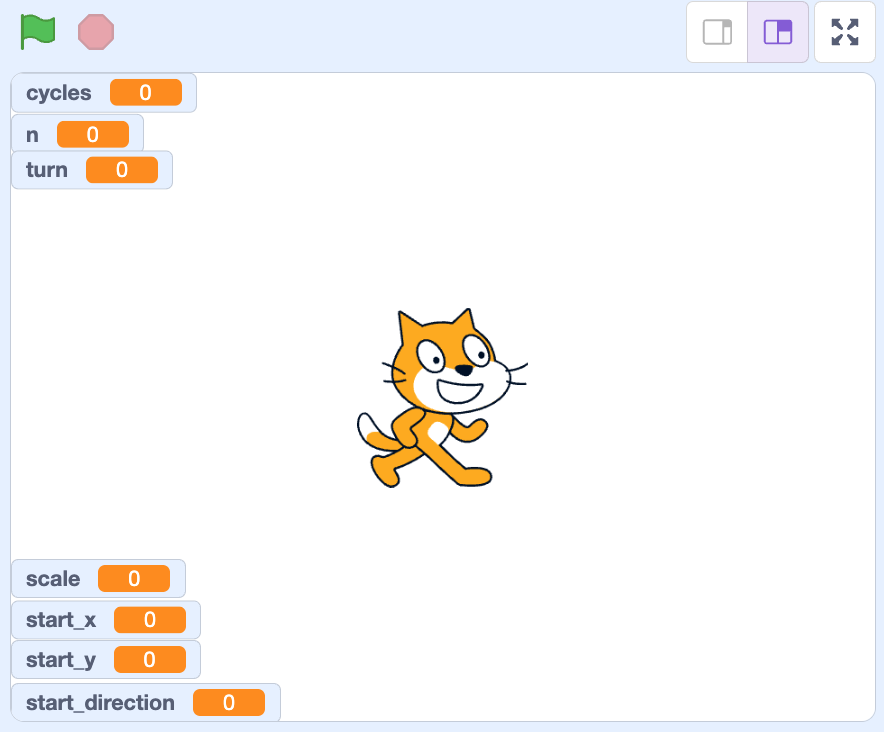
\includegraphics[width=0.5\textwidth,height=\textheight]{readouts.png}
  \end{itemize}
\item
  Start the code. In the left-most frame, find the correct elements, and
  drag them into place.

  \begin{itemize}
  \tightlist
  \item
    After ``Space'' is hit: set the parameters, clear the previous
    drawings, lift the pen, move the pen to the initial position and
    direction, and put the pen back down.
  \item
    You will \textbf{set the paramters here} for each drawing.\\
    
\includegraphics[width=\textwidth,height=0.6\textheight]{code_01.png}
    \newpage
  \end{itemize}
\item
  Code the drawing loop. (All the code from steps 5 and 6 is together in
  one chunk.)\\
  
\includegraphics[width=\textwidth,height=0.4\textheight]{code_02.png}
\item
  Code a new chunk to interrupt the drawing by pressing ``x''.\\
  \includegraphics[width=0.3\textwidth,height=\textheight]{stopall.png}
\item
  Hide the sprite. (Hide the cat.)

  \begin{itemize}
  \tightlist
  \item
    Near the bottom-right frame, click the show/hide sprite toggle.\\
    
\includegraphics[width=0.2\textwidth,height=\textheight]{hide_sprite.png}
  \end{itemize}
\item
  If your code gets busted, you can use mine:
  \url{https://scratch.mit.edu/projects/1214544750}
\end{enumerate}

\newpage

\begin{enumerate}
\def\labelenumi{\arabic{enumi}.}
\setcounter{enumi}{9}
\tightlist
\item
  \textbf{DOCUMENT} your own patterns in a slideshow!

  \begin{itemize}
  \tightlist
  \item
    Adjust the parameters in the top of the code, press space bar to run
    the code.

    \begin{itemize}
    \tightlist
    \item
      The main parameters are \texttt{countdown\_max} and
      \texttt{direction\_change}. These fundamentally alter the pattern
      drawn.
    \item
      The other parameters allow you to scale and move the drawing.
    \end{itemize}
  \item
    \textbf{DO NOT} let drawing hit edge of screen. Use a smaller
    \texttt{scale} value if this happens.
  \item
    Try to make the drawing as large as possible without hitting the
    edge of the window or going behind the readouts.
  \item
    Try to center the image horizontallyuyi65t by adjusting the
    \texttt{x\_inital} value.
  \item
    Try to center the image vertically by adjusting the
    \texttt{y\_inital} value.
  \item
    \textbf{Document your best patterns}.

    \begin{itemize}
    \tightlist
    \item
      Start a new slideshow. Use \href{https://slides.new}{slides.new}
      for google slides.
    \item
      For a title page, include your name, date, and a title\ldots{}
      something like ``Countdown Spirals''
    \item
      When you have a high-quality spiral, take a screenshot including
      the readouts. Paste the screenshot into the slideshow as its own
      slide.
    \item
      Before taking a screenshot, go to full-screen mode.
      \includegraphics[width=0.05\textwidth,height=\textheight]{fullscreen.png}
      (Button near top-right.)
    \end{itemize}
  \end{itemize}
\item
  You can see an exemplar here:

  \begin{itemize}
  \tightlist
  \item
    \url{https://chadworley.github.io/pbl/scratch/exemplar.html}
  \end{itemize}
\end{enumerate}

\end{document}
